\section{Introduzindo as Imagens HDR ao Processo} \label{pontosProcesso}

Dentre os softwares de geração de nuvem de pontos pesquisados, nenhum possui suporte para leitura e processamento de imagens HDR. Esta problemática exige uma solução alternativa para que seja possível o uso das informações contidas nas imagens HDR para obtenção de nuvem de pontos. Assim como Kontogianni~\etal~\cite{hdr3d} e P\v{r}ibyl~\etal~\cite{hdr3d2}, foi decidido pelo uso de imagens HDR processadas com técnicas de tone mapping para geração de uma imagem LDR com mais detalhes e então prosseguir com a obtenção da nuvem de pontos.

\subsection{Método de Tone Mapping} \label{pontosToneMapping}

Como citado na Seção \ref{baseImgPicturenaut}, o Picturenaut possui uma ferramenta mapear tons de uma imagem HDR. Esta funcionalidade é usada para efetuar o tone mapping das imagens HDR com as configuraçõe de filtro bilateral, contraste máximo, e saturação máxima. Essas configurações aumentam a preservação dos detalhes e contraste entre os pixels da imagem processada. A Figura \ref{pontosToneMapping} exemplifica a configuração do tone mapping de uma imagem.

\begin{figure}[H]
  \centering
  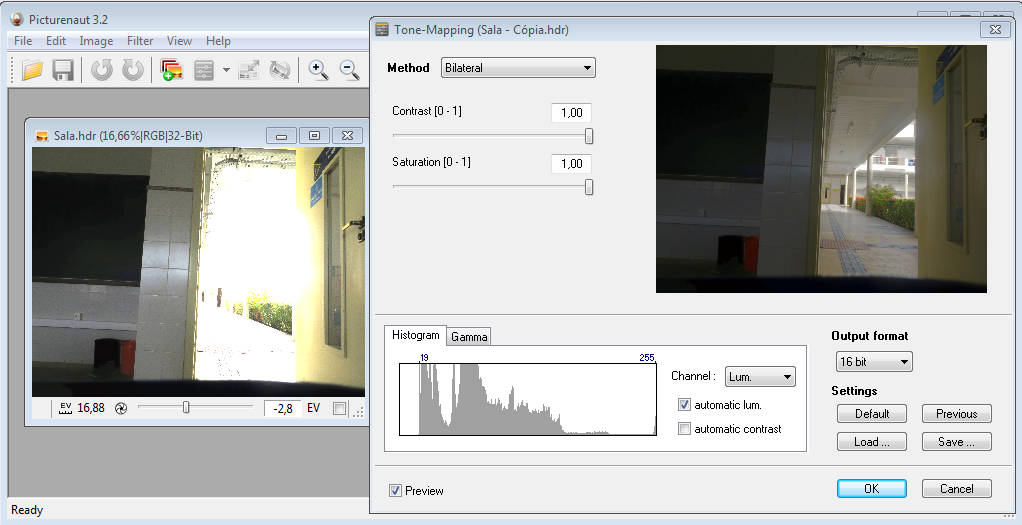
\includegraphics[height=8cm]{salaToneMapped}
  \caption{Exemplo de imagem HDR tonemapped.}
  \label{figExemploSFM}
\end{figure}